\documentclass[10pt]{article}

% Language setting
\usepackage[english]{babel}

% Set page size and margins
% Replace `letterpaper' with`a4paper' for UK/EU standard size
\usepackage[a4paper,top=4.44cm,bottom=3.17cm,left=2.12cm,right=2.12cm]{geometry}

% Useful packages
\usepackage{tabularx} % Add this in the preamble
\usepackage{amsmath}
\usepackage{booktabs}
\usepackage{graphicx}
\usepackage[colorlinks=true, allcolors=blue]{hyperref}
\usepackage{paralist} % For inline enumerate and itemize
\usepackage{enumitem} % For more control over list environments
\usepackage{subcaption}
\usepackage[style=numeric,sorting=none]{biblatex}
\addbibresource{reference.bib} % Add your bibliography file here
\usepackage{newtxtext} % Modern Times New Roman font
\usepackage{geometry} % For custom margins
\usepackage{setspace} % For line spacing
\usepackage{parskip} % For paragraph spacing control
\usepackage{indentfirst} % To indent the first line of each section
\setlength{\parindent}{0.51cm} % First-line indentation
\setlength{\parskip}{6pt} % Paragraph spacing

\pdfminorversion=5
\pdfobjcompresslevel=0
\pdfcompresslevel=0

\title{\fontsize{14pt}{16pt}\selectfont Synthetic Data Enhances Mathematical Reasoning of Language Models}
\author{
    Zeyu Han\textsuperscript{1,*} \and First Name Last Name\textsuperscript{2}
}

\begin{document}
\maketitle

\begin{center}
\begin{minipage}{0.8\textwidth}
\begin{center}
\textbf{Abstract}
\end{center}
Current large language models (LLMs) training involves extensive training data and computing resources to handle in multiple natural language processing (NLP) tasks. This paper endeavors to assist individuals to compose feasible mathematical question-answering (QA) language models in specific fields. We leveraged Gretel.ai, a feasible data generation platform, to generate high-quality mathematical QA data covering several areas, including definitions, theorems, and calculations related to linear algebra and abstract algebra. After fine-tuning through \textsc{Open-AI} infrastructure, GPT-3 performed  significant improvements on accuracy, achieving an roughly 18.2\% increase in abstract algebra benchmark, approximately 1.6x improvement on linear algebra theorems benchmark, and approximately 24.0\% increase on linear algebra calculations benchmark. And small language models (SLMs) such as \textsc{LLama-2-7B/13B} and \textsc{Mistral-7B} have outstanding around 2x accuracy advancements in linear algebra calculations. This study demonstrates the potential for individuals to develop customized SLMs for specialized mathematical domains using synthetic data generation and fine-tuning techniques. Our fine-tuned SLMs are available at \href{https://huggingface.co/Charlie-Han-01}{https://huggingface.co/Charlie-Han-01}, and project page is available at \href{https://github.com/DinoZeyu/LLM-Research.git}{https://github.com/DinoZeyu/LLM-Research.git}.
\end{minipage}
\end{center}

\begin{center}
\begin{minipage}{\textwidth}
\textbf{Keywords:} AI generated data; artificial intelligence;text classification; data collection cost; mathematical question-answering; downstream task training
\end{minipage}
\end{center}

\section{Introduction}\label{sec:1}
In recent years, there has been a significant improvement in NLP and LLMs techniques to increase the comprehensive ability and generalization of models. From word embedding models  
 \cite{Mikolov2013EfficientEO,Pennington2014GloVeGV} to Transformer based encoder and decoder autoregressive models  
  \cite{devlin2019bertpretrainingdeepbidirectional, Raffel2019ExploringTL, Brown2020LanguageMA, Chowdhery2022PaLMSL, touvron2023llamaopenefficientfoundation, Touvron2023Llama2O}, the flourishing progress of LLMs depends on appearance of Transformer structure \cite{Vaswani2017AttentionIA}, innovation of effective finetuning algorithms and techniques \cite{Kwon2023EfficientMM,Dao2022FlashAttentionFA,Hu2021LoRALA,Dettmers2023QLoRAEF}, and the gradually increasing diversity and scale of training data.\\ 

In order to improve the ability of LLMs, \cite{kaplan2020scalinglawsneurallanguage} indicated that the model's performance could be enhanced by increasing its parameters to enlarge the model size to improve performance according to abundant database. However, the cost of computational resources, primarily GPUs, and data collection increases proportionally with the size of the model. Fine-tuning a sparse Mixtral model with 2M queries may require a NVIDIA H100 GPU with cost of \$3460 \cite{xia2024understandingperformanceestimatingcost}. And pre-training a LLM is substantially more expensive, sometimes reaching millions of dollars, due to requirements of GPU clusters, massive dataset, and electric consumption. Taking GPT-3 175B \cite{Brown2020LanguageMA} as an example, it is trained on V100 GPU high-bandwidth clusters with mixed datasets composed of CommonCrawl \cite{Raffel2019ExploringTL} and WebText \cite{radford2019language} totaling nearly 430 billion tokens and its training expenses exceed $\$4.6$ million \cite{lambda_demystifying_gpt3}.\\

Meanwhile, data quality has became an area of concern. In the case of unsupervised pre-training, the quality of training data involved in few-shot learning process would greatly affect the performance of LLMs, thus influencing the generalization and adaptability of models to different downstream tasks \cite{Brown2020LanguageMA}. Similarly, training LLMs with adequate AI generated NLP feedback data and efficient parametric fine-tuning technique LoRA \cite{Hu2021LoRALA} could effectively improve the performance of QA task in low-data scenarios \cite{li2023laffileveraginghybridnatural}. \\

Therefore, this paper initially proposes to address the downstream task by utilizing AI generated high-quality data to verify the effectiveness of our method in QA of mathematical definitions, theorems and calculations. On the one hand, our method could effectively reduce the costs associated with data collection, data cleaning, and computing resources. On the other hand, individuals could train small mathematical language models to fulfill personal demands.\\

Since data plays a crucial role in the fine-tuning process of downstream tasks for LLMs, the performance of models typically shows a monotonic increasing trend with the alignment degree between pre-training data and downstream task fine-tuning data \cite{isik2024scalinglawsdownstreamtask}. In order to effectively align the downstream task data with the large amount of pre-trained data, the followings should be noted: \begin{inparaenum}[(i)] \item Include the relevant areas of specific targets \cite{wei2022finetunedlanguagemodelszeroshot}; \item Ensure the diversity and accuracy of data, in other words, data quality \cite{Li2023FromQT}. \end{inparaenum} Our method could adequately explore the generalization of LLMs to ensure the performance of SLMs for specific task. Compared to LLMs, SLMs could achieve even or better performance with less computational resources, time, and size of dataset. For example, there are some highly effective BERT-based SLMs:DistilBERT \cite{sanh2020distilbertdistilledversionbert}, ALBERT \cite{DBLP:journals/corr/abs-1909-11942}, TinyBERT \cite{jiao2019tinybert}, and MiniLM \cite{wang2020minilm}. SLMs improve their performance by learning the self-attention mechanism of LLMs during the training process, forming a relationship similar to that of a teacher and students \cite{wang2020minilmdeepselfattentiondistillation,Liang2023LetGB}. Fine-tuning LLMs with a fewer well-filtered dataset, i.e., instruction fine-tuning data \cite{Li2023FromQT}, is a practical approach that can enable the model to achieve SoTA performance on various tasks \cite{Chen2023AlpaGasusTA}. \\
 
Notably, \cite{kojima2023largelanguagemodelszeroshot} conducted a study combining a simple prompt template with few-shot learning, which allowed models to gradually analyze answers and inference logic to effectively improve the models' problem-solving ability and accuracy of outputs.  In addition, \cite{Wang2022PromDAPD} proposed that using prompt-based data augmentation could ensure the quality of synthetic data which would increase the natural language understanding of models.
\\
 
Prior researches have indicated that fine-tuning mathematical tasks using AI generated instructions for existing datasets would accelerate the reasoning process and enhance model's performance. Our contributions could be summarized as follows:
\begin{itemize}
    \item Integrate the instructions directly into data generation process which provides models with elaborate procedures of problem-solving, and facilitate customized datasets tailored to individual requirements. 
    \item Reduce the costs of fine-tuning models by simplifying data collection and lowering the requirements for computational resources. 
    \item Improve the accuracy of models in mathematical QA after fine-tuning and explore the influence of model choices to their performance. 
\end{itemize}

\section{Related Works}
\subsection{LLM Overview}
In recent years, general multimodal LLMs have an impressive development in many areas of NLP such as BERT series \cite{devlin2019bertpretrainingdeepbidirectional}, T-5 \cite{Raffel2019ExploringTL}, Megatron-Turing NLG \cite{smith2022usingdeepspeedmegatrontrain}, LLaMA series \cite{Touvron2023Llama2O}, ChatGPT series \cite{openai2024gpt4technicalreport}, PaLM \cite{chowdhery2022palmscalinglanguagemodeling}, and these models have outstanding performance on many NLP tasks as shown in Figure~\ref{fig:timeline}. Meanwhile, these models also have corresponding SLMs such as GPT-4o mini \cite{openai_gpt4omini_2024}, LLama-2-7B/13B \cite{touvron2023llamaopenefficientfoundation}, and TinyLlama \cite{zhang2024tinyllamaopensourcesmalllanguage}. However, these models may be unsatisfactory in some mathematical QA tasks or details. For example, \textbf{ChatGPT 4o} may could not correctly recognize which number is larger as shown in Figure~\ref{fig:math error}. 
\begin{figure}[h]
    \centering
    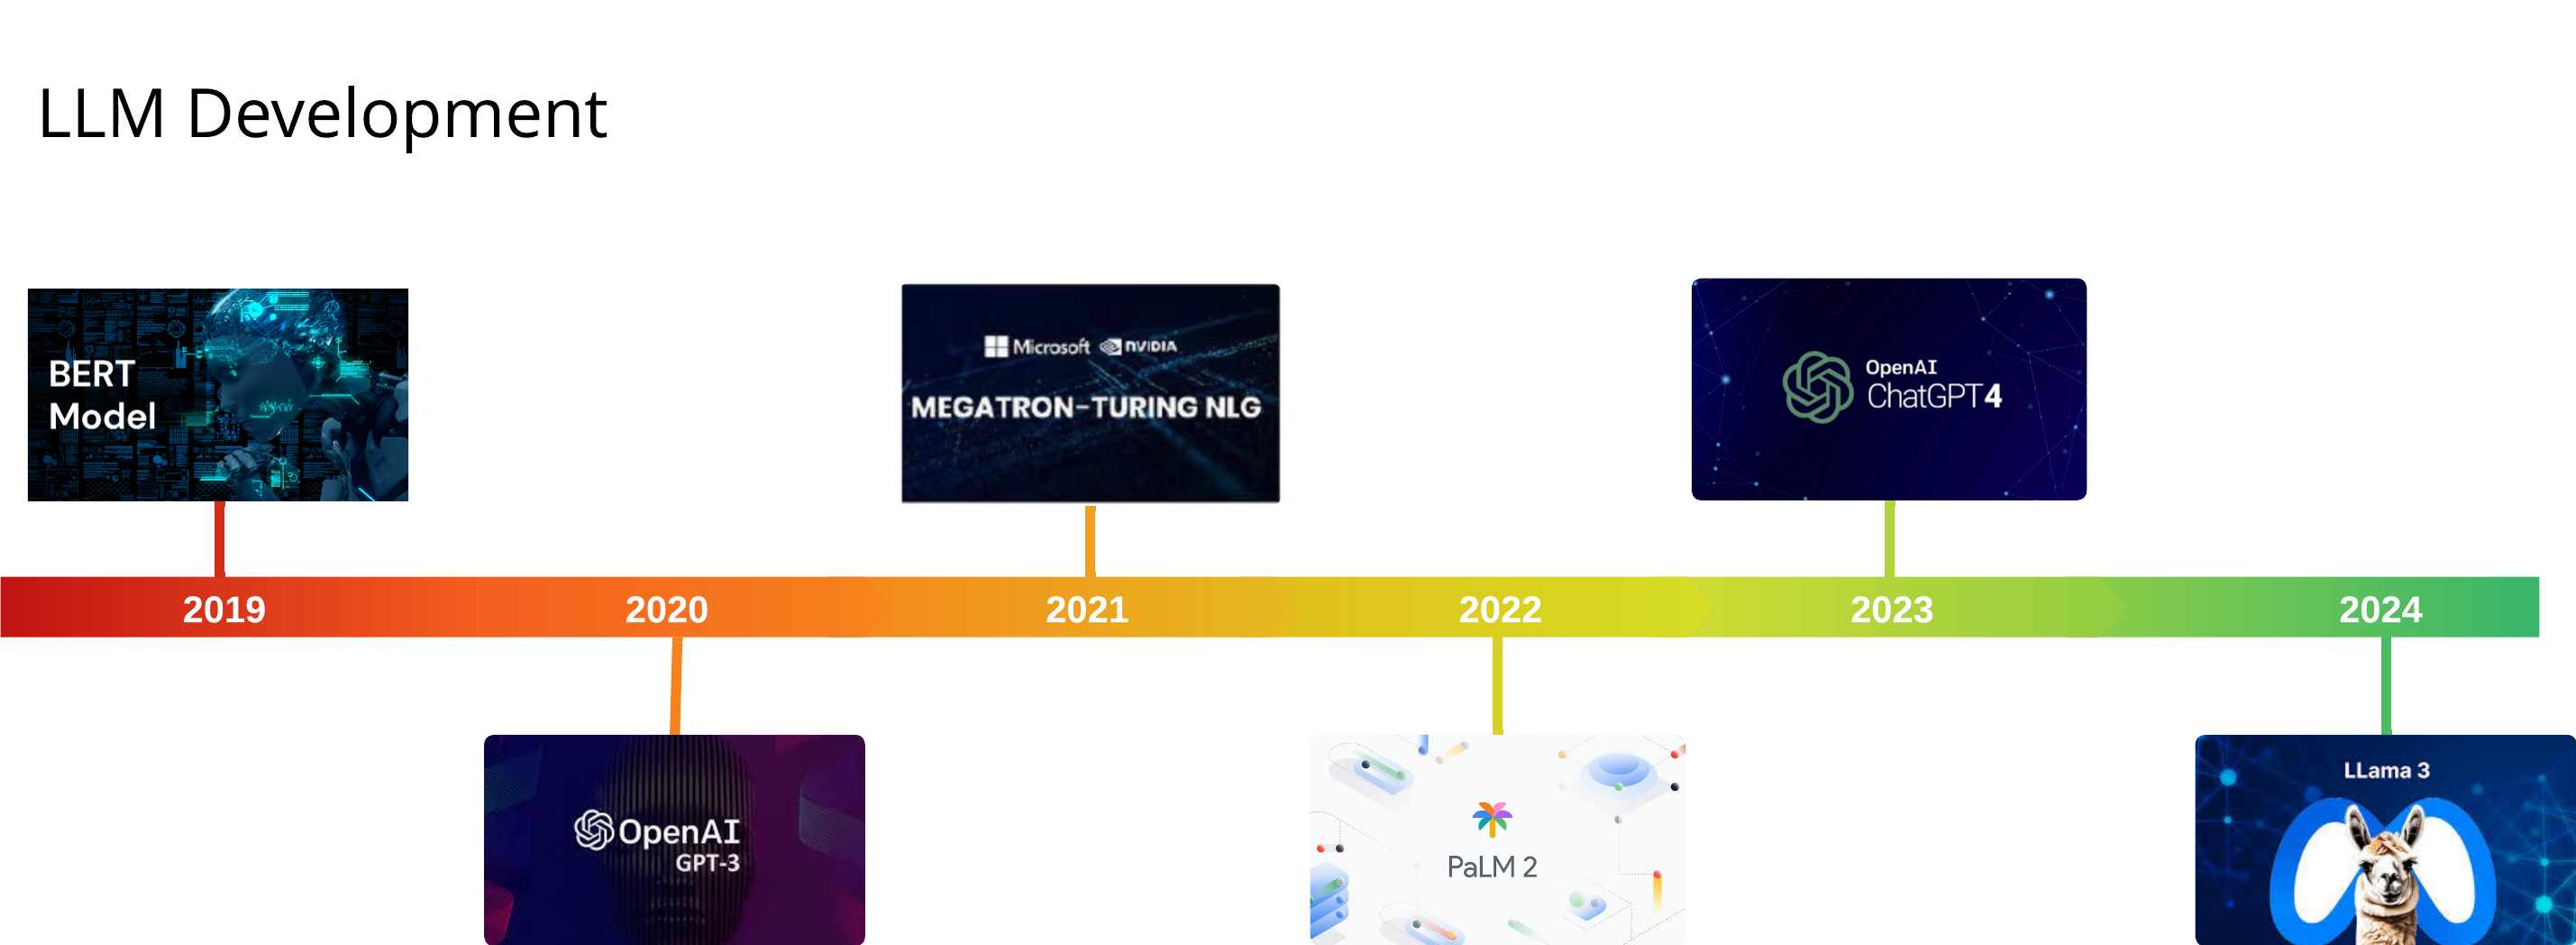
\includegraphics[width=\linewidth]{Figures/LLM timeline.png}
    \caption{Recent years representative LLMs which achieve SoTA performance during their periods. \textbf{\textsc{BERT}} \cite{devlin2019bertpretrainingdeepbidirectional} initially used bidirectional Transformer architectures. \textbf{\textsc{T-5}} \cite{Raffel2019ExploringTL} proposed to covert NLP tasks into a text-to-text form. \textbf{\textsc{GPT-3}} \cite{Brown2020LanguageMA} performed excellent effectiveness of few-shot and zero-shot learners and made a wide influence. \textbf{\textsc{PaLM}} \cite{chowdhery2022palmscalinglanguagemodeling} strongly validated the Scaling Laws in LLMs pre-training. \textbf{\textsc{GPT-4}} \cite{openai2024gpt4technicalreport} and \textbf{\textsc{LLama3}} \cite{dubey2024llama3herdmodels} are the most popular and well-known LLMs present days due to their high performance.}
    \label{fig:timeline}
\end{figure}

\begin{figure}[h]
    \centering
    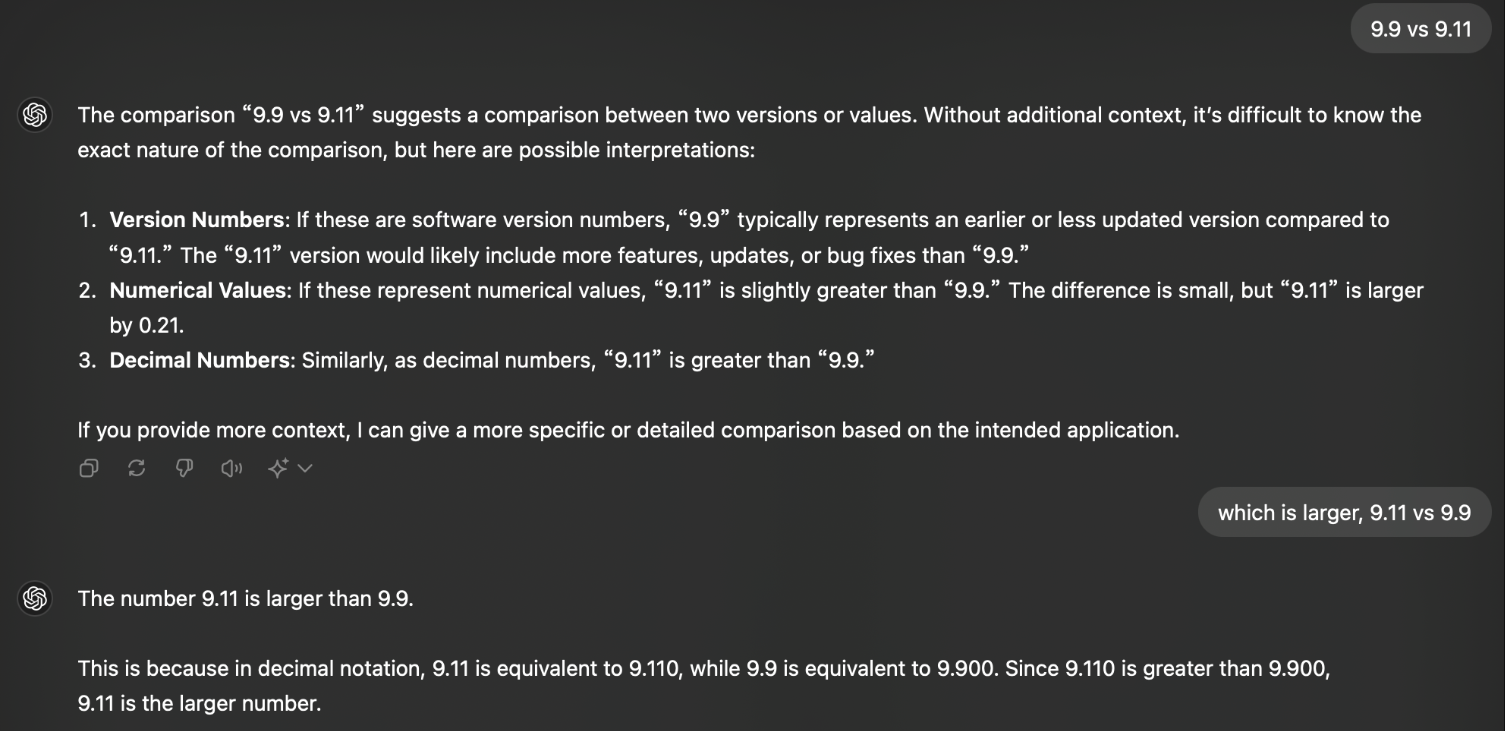
\includegraphics[width=0.8\linewidth]{Figures/GPT4o math error.png}
    \caption{\textbf{ChatGPT 4o} sometimes may have confusion to figure out which number is larger, 9.11 or 9.9.}
    \label{fig:math error}
\end{figure}

\subsection{Math-Related Models}
 
 
With the rapid advancement of LLMs, mathematical problem-solving capability has emerged to be one of critical standards to evaluate the effectiveness and efficiency of LLMs. Based on well-curated pre-trained LLMs, researchers have developed multiple effective techniques to finetune models specifically for mathematically downstream tasks or building SLMs.\\
\\
\textbf{AlpaGasus:} Developed by \cite{Chen2023AlpaGasusTA}, the AlpaGasus model represents a feasible technique that utilizing powerful LLMs to mitigate the performance reduction of Alpaca \cite{alpaca} caused by the misleading and detrimental IFT data. In addition, AlpaGasus achieves a remarkable cost saving which reaches \$4.78 lowest for a 7B model. It emphasizes the significance of data quality for model performance.
\\
\\
\textbf{MAmmoTH:} As an instruction tuning based math model, MAmmoTH \cite{Yue2023MAmmoTHBM} primarily enhanced the general mathematical reasoning ability according to train the model on a dataset called MathInstruct that covers multiple mathematical areas and corresponding hybrid rationales. The model's performance on general math benchmarks \cite{hendrycksmath2021, Cobbe2021TrainingVT,Ling2017ProgramIB} has a significantly improvement compared to other open source models such as WizardMath  \cite{luo2023wizardmathempoweringmathematicalreasoning}. 
\\
\\
\textbf{MathBERT:} Unlike other models, MathBERT \cite{Peng2021MathBERTAP} focused on the structures of formulas and their corresponding contexts to strengthen the semantic understanding of mathematical formulas of the model during pre-training process. According to pre-training model on data including formula with context, MathBERT has demonstrated high relevance score on NCTIR-12 \cite{Zanibbi2016NTCIR12MT} benchmark and remarkable precision and recall on TopicMath-100K \cite{Peng2021MathBERTAP} benchmark. It performed outstanding results on mathematical information retrieval, formula topic classification and formula headline generation downstream tasks.
\\
\\
\textbf{o1-mini:} In September 14th 2024, \textsc{OpenAI} released the \textsc{o1-mini} model \cite{openai2024o1mini} which made an progressive advancement in cost-efficient reasoning capabilities in mathematics. Notably, \textsc{o1-mini} has outperformed both \textsc{GPT-4o} and \textsc{GPT-4o-mini} on the AIME benchmark, while also offering a more economical inference cost than \textsc{o1} and \textsc{o1-preview}.  Furthermore, \textsc{o1-mini} is 3 to 5 times faster than \textsc{o-1 preview} with correct answers compared to \textsc{GPT-4o}. However, the cost of \textsc{o1-mini API} would be \$1000 which is expensive for individuals.   
\\
Our paper leverages the convenience and effectiveness of mathematical text generation in LLMs and cheapness of cloud computing to finetune task specific model with limited conditions for individuals. From an expenditure perspective, our method skips the instruction filtering step and straightforwardly generates high quality data compared to AlpaGasus \cite{Chen2023AlpaGasusTA} which avoids additional time consumption and charges. From an academic perspective, our method concentrates on the particular mathematical task which may be more optimal for individuals to develop a model to meet specific requirements in contrast to MAmmoTH \cite{Yue2023MAmmoTHBM} and MathBERT \cite{Peng2021MathBERTAP}.  

\section{Data Description}\label{sec:data}
\begin{figure}[h]
    \centering
    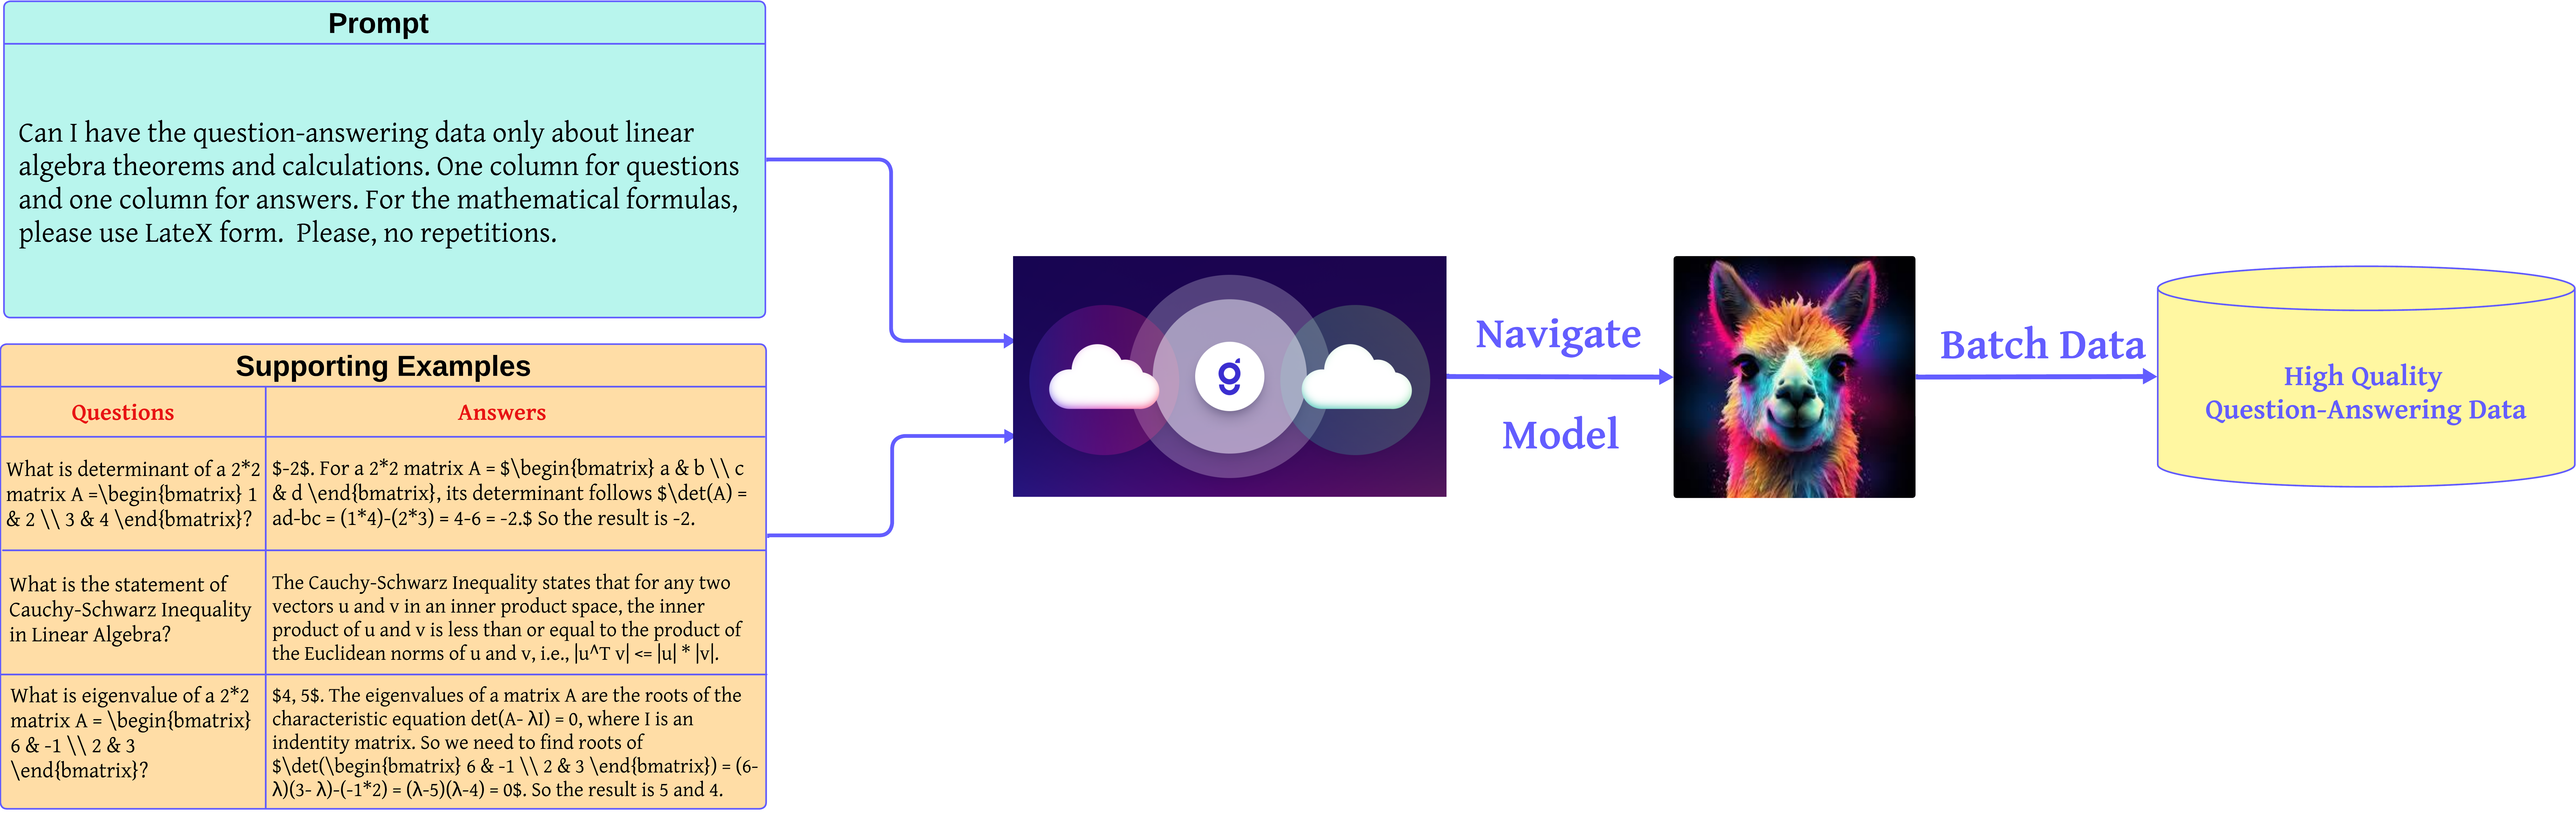
\includegraphics[width= \linewidth]{Figures/Data Generation LLama.png}
    \caption{Data generation platform \textsc{Gretel.ai}. We provide the prompt and sample data for \textsc{Gretel.ai} cloud to create navigator model. According to navigator, the platform chooses the \textsc{Gretel-Llama-3.1-8B-Instruct} model to batch synthetic linear algebra data.}
    \label{fig:data generation}
\end{figure}
\subsection{Fine-Tuning Data}\label{sec:3.1}
The dataset used to fine-tune the models is composed of three curated datasets with theorems and calculation of mathematics: one primarily focuses on linear algebra theorem problems (5000 rows), another on computational problems of linear algebra (3000 rows), and the third containing 3000 abstract algebra problems.\\
\begin{figure}[h]
    \centering
    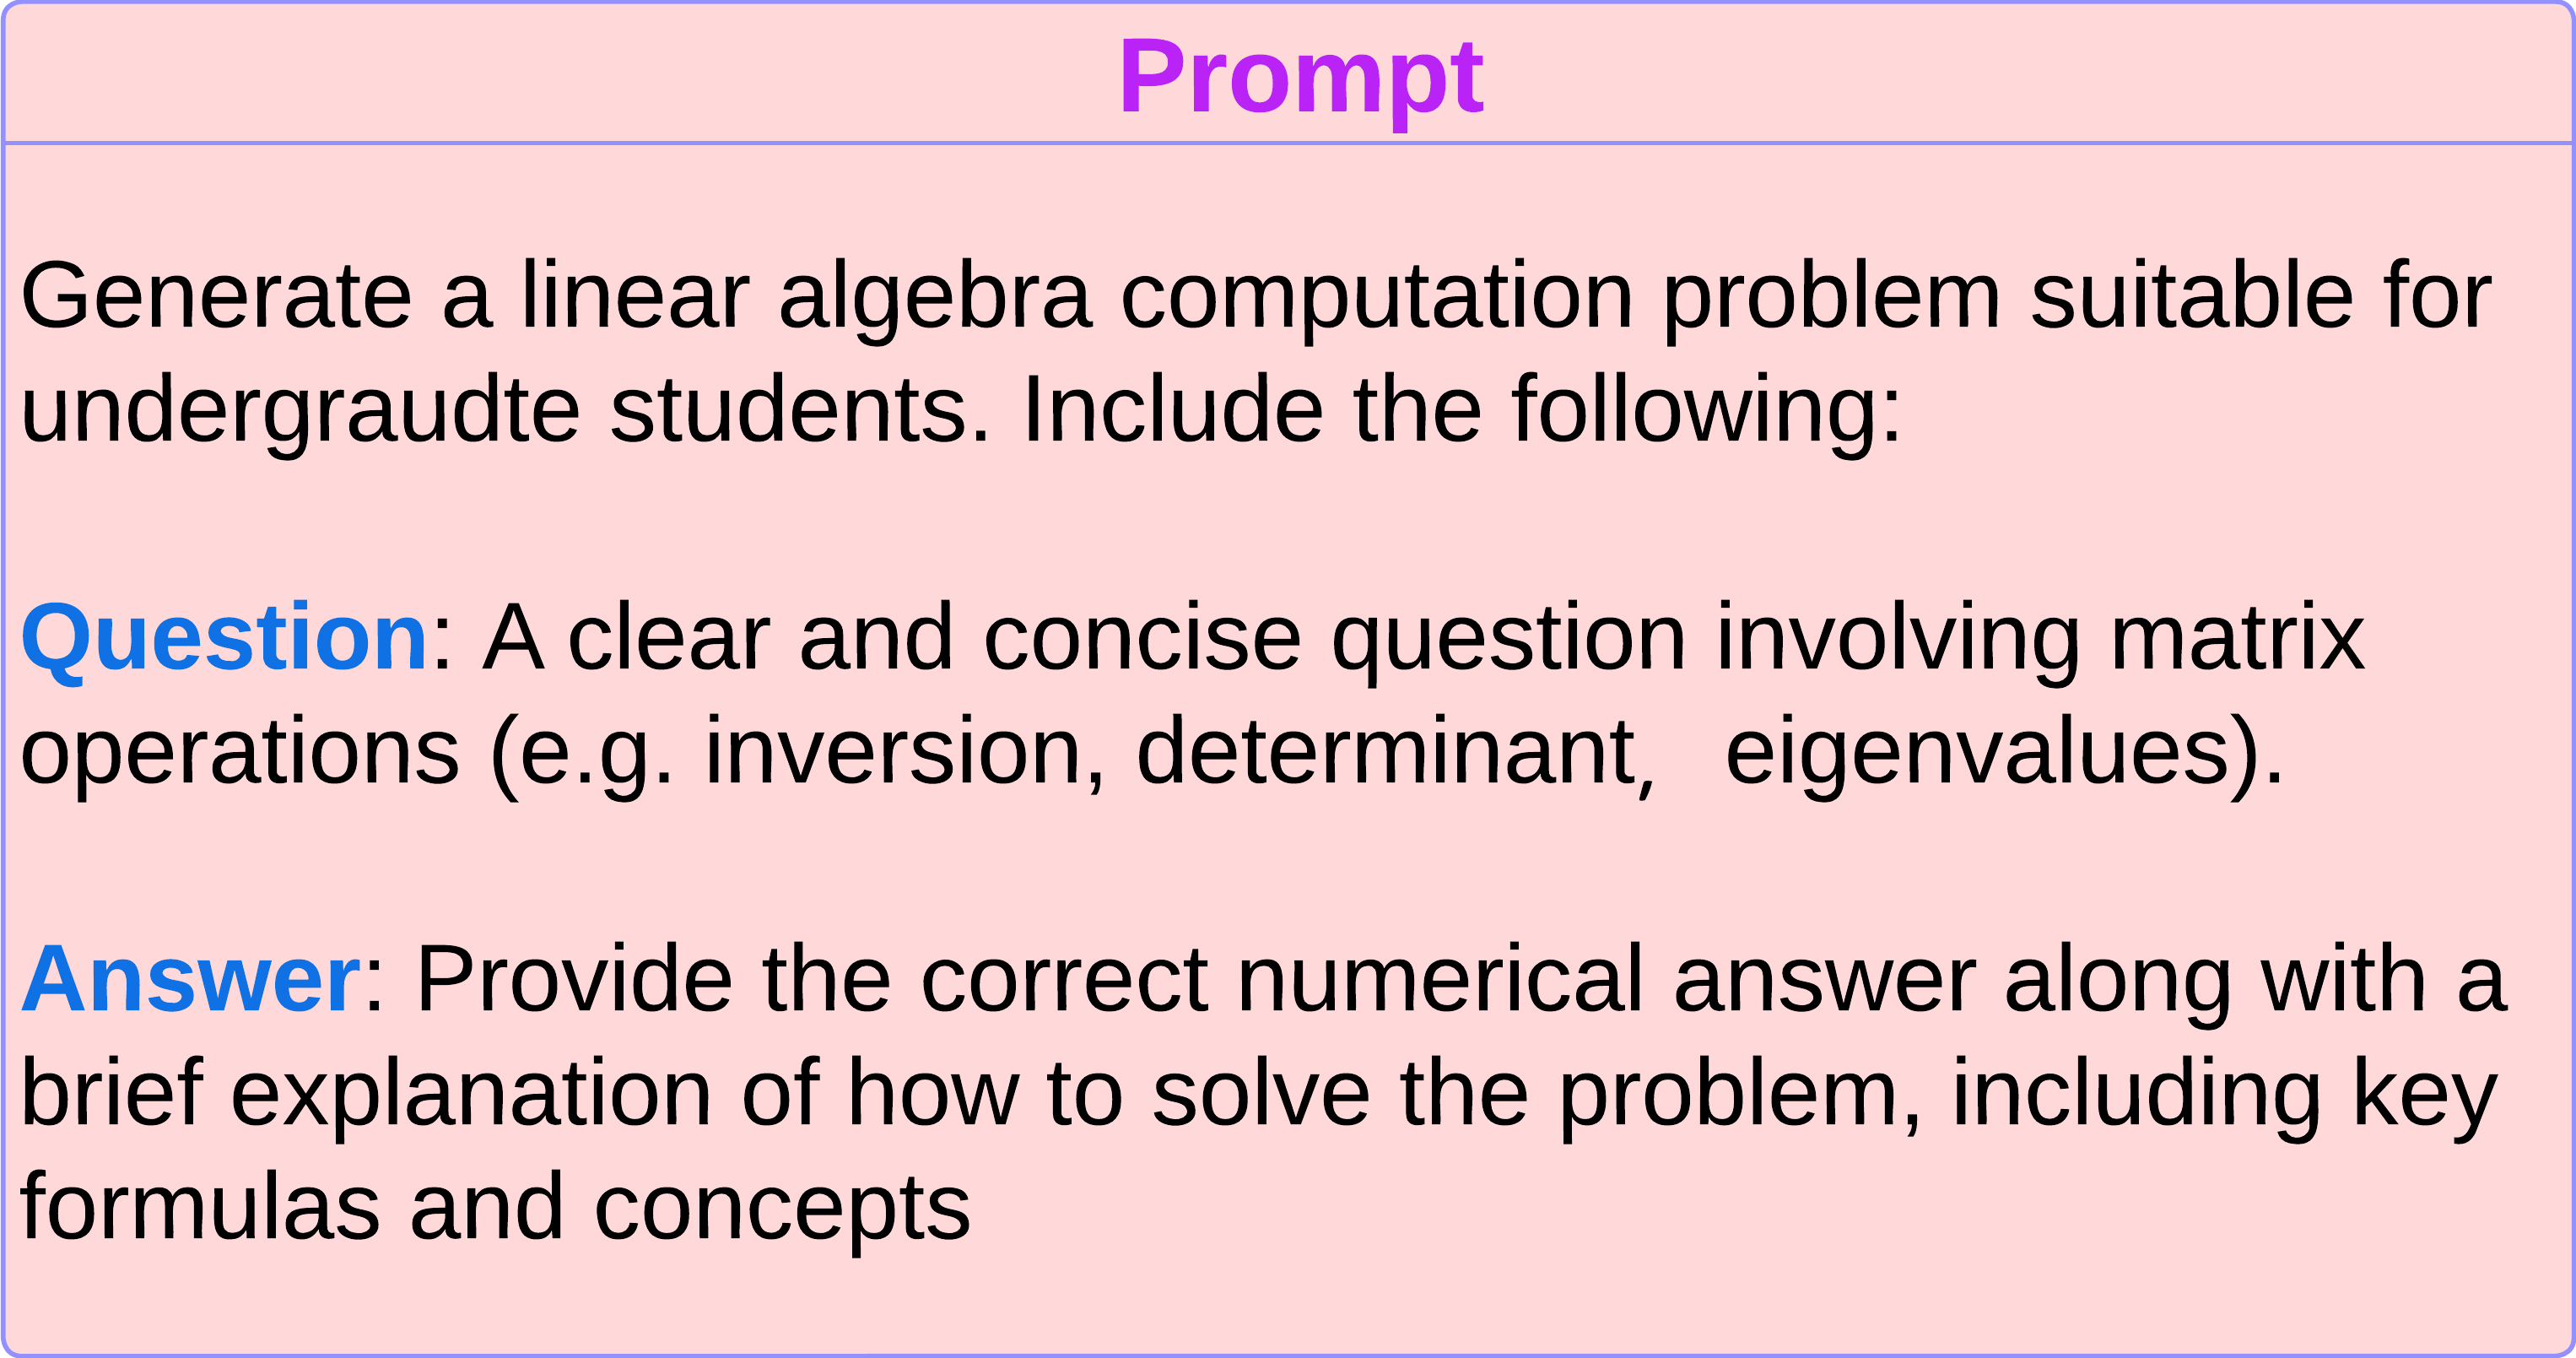
\includegraphics[width=0.6\linewidth]{Figures/Calculation Prompt.png}
    \caption{Prompt to synthesize Linear Algebra Computation QA Data }
    \label{fig:cal prompt}
\end{figure}

For the data generation process, as shown in Figure~\ref{fig:data generation}, we initially refined our requirements for synthetic data according to an elaborate prompt, and examples covering theorems and calculations pertinent to the specific mathematical field. Then, the \textsc{Gretel.ai} platform generated 100 rows of tabular data with parameters $T = 1.0$(temperature controlling the randomness of generation), $K = 40$(number of highest probability tokens considered for generation), and $P = 1.0$ (cumulative probability threshold for token selection) to maximize the variability in generated data. Subsequently, the platform leveraged existing prompt and data to construct a navigator model capable of selecting appropriate fine-tuned models and generating data in batches as required. The linear algebra data was generated from Gretel-LLAMA-3.1-8B \cite{MetaLLaMA31} and abstract algebra data was generated from Gretel GPT-3.5 Turbo \cite{OpenAIGPT35TurboFineTuning}. In addition, we have standardized the mathematical formulas into LaTeX format to guarantee consistency. \\

Nevertheless, we observed that the linear algebra dataset contains few computational problems and corresponding solutions. Although language models possess zero-shot learning capabilities \cite{Brown2020LanguageMA}, the lack of computation section would reduce the models' performance significantly. Therefore, we also used \textsc{Gretel-LLAMA-3.1-8B} with parameters $T = 0.9$, $K = 35$, and $P = 0.8$ to synthesize linear algebra calculation dataset including reasoning process containing necessary concepts and formulas according to effective prompt design as shown in Fig~\ref{fig:cal prompt}, which could be considered as data augumentation \cite{ding2024dataaugmentationusinglarge}. \\
\\
\begin{figure}[h]
    \centering
    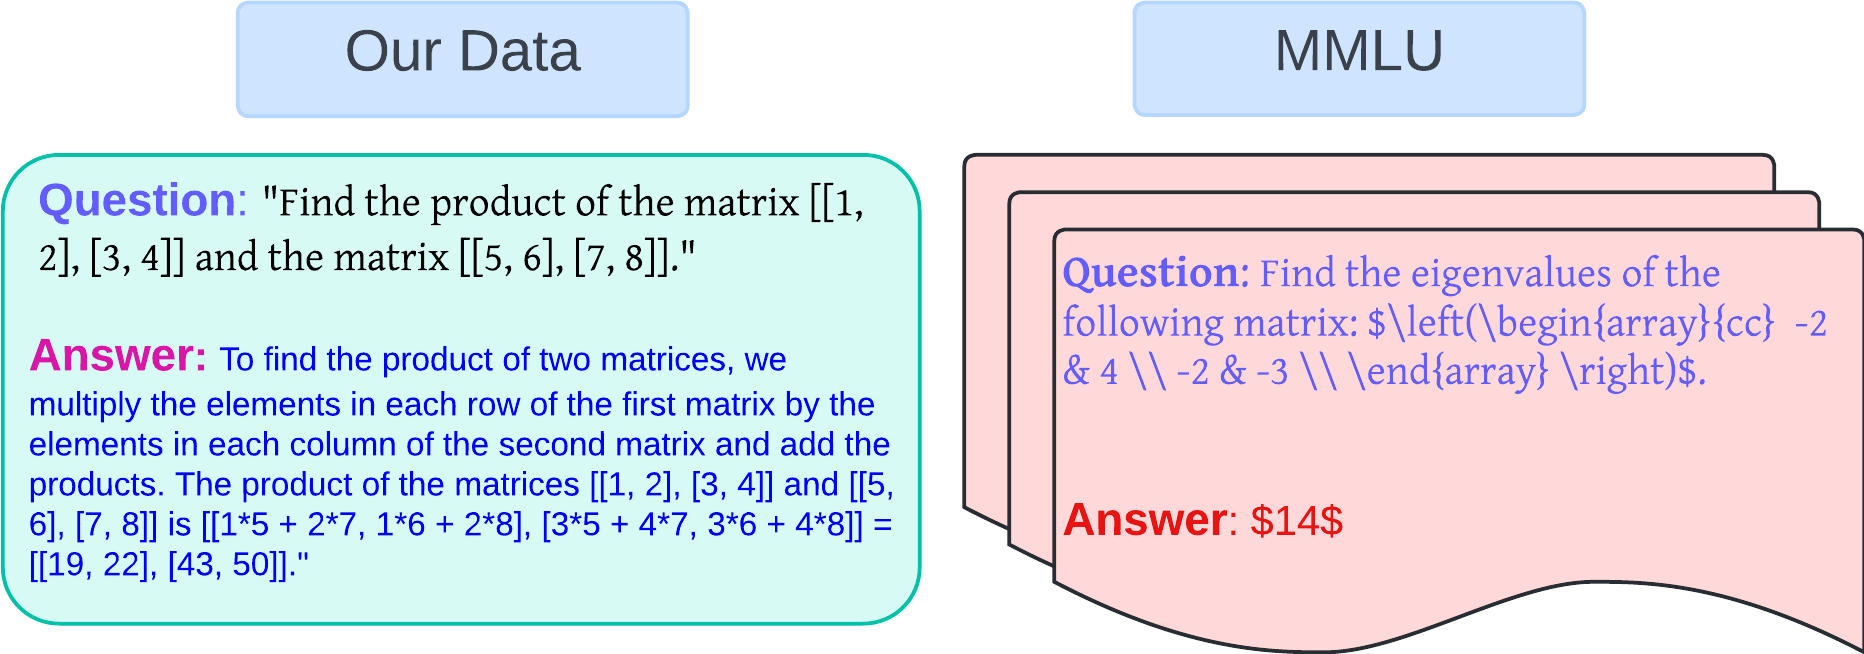
\includegraphics[width=0.9\linewidth]{Figures/Data Comparision.png}
    \caption{Data difference between two datasets. In our dataset, we included the process of solving problems, which is similar to chain-of-thought \cite{wei2023chainofthoughtpromptingelicitsreasoning} to get outputs compared to MMLU.}
    \label{fig:data comparision}
\end{figure}

 
In contrast to prior research \cite{Chen2023AlpaGasusTA, Yue2023MAmmoTHBM, kojima2023largelanguagemodelszeroshot}, our data generation method provides individuals with a feasible approach to obtain cost-effective high quality data, as shown in Figure~\ref{fig:data comparision}, for fine-tuning customized models. The total time to generate the data was approximately three hours without any expenses since the \textsc{Gretel.ai} provides all users free 1.5 million characters usage per month. 

\subsection{Benchmarks}\label{sec:3.2}

\begin{table}[ht]
\centering
\small % Reduce font size slightly
\renewcommand{\arraystretch}{1.3} % Adjust vertical spacing
\setlength{\tabcolsep}{8pt} % Adjust horizontal spacing for clarity
\begin{tabularx}{\textwidth}{p{3.5cm} l c c} % Set specific width for "Datasets" column
\toprule
\textbf{Datasets} & \textbf{Source} & \textbf{Size} & \textbf{Usage} \\
\midrule
\parbox[t]{3.5cm}{Linear Algebra} & Gretel LLAMA-3.1-8B & 5.0k & Fine-tuning \\
\parbox[t]{3.5cm}{Abstract Algebra} & Gretel GPT-3.5-Turbo & 3.0k & Fine-tuning \\
\parbox[t]{3.5cm}{Linear Algebra Calculation} & Gretel LLAMA-3.1-8B & 1.0k & Fine-tuning \\
\midrule % Insert horizontal line to separate the sections
\parbox[t]{3.5cm}{Theorem QA} & \cite{Chen2023TheoremQAAT} & 52 & Evaluation \\
\parbox[t]{3.5cm}{MATH} & \cite{hendrycksmath2021} & 2.0k & Evaluation \\
\parbox[t]{3.5cm}{Linear Algebra QA} & \cite{Likhi2003_linearalgebra_QA} & 223 & Evaluation \\
\parbox[t]{3.5cm}{Partial MMLU} & \cite{hendrycks2021ethics} & 101 & Evaluation \\
\bottomrule
\end{tabularx}
\caption{Overview of datasets and benchmarks used in the experiments.}
\label{tab:benchmark}
\end{table}

 
In order to examine the feasibility of our fine-tuning method, we chose widely used mathematical benchmarks and take samples from them to evaluate the performance of fine-tuned models accuracy on these benchmarks. The specific datasets we used are listed in Table \ref{tab:benchmark}.\\
\\
\textbf{TheoremQA} \cite{Chen2023TheoremQAAT} is designed for evaluating the models' mathematical reasoning ability to apply theorems into specific question to deduce the correct answer. Since it lacks a dedicated linear algebra section, we utilized human evaluation to filter the satisfactory linear algebra data from algebra portion as test set. \\
\\
\textbf{MATH} \cite{hendrycksmath2021} is a widely used benchmark for evaluating the mathematical reasoning abilities of LLMs. It contains various areas including precalculus, algebra, geometry, and number theory, among others, as test datasets. However, the original MATH dataset does not include linear algebra QA data. In order to address this drawback and evaluate linear algebra ability of fine-tuned models, we randomly selected 1000 eigenvalue problems and determinant problems equally from the linear algebra portion of AMPS pretraining dataset where you can find it {\href{https://drive.google.com/file/d/1hQsua3TkpEmcJD_UWQx8dmNdEZPyxw23/view?usp=sharing}{here}} as a dedicated test set.\\
\\
\textbf{Linear Algebra QA} \cite{Likhi2003_linearalgebra_QA} dataset categorizes the difficulty of problems into five levels and provides direct answers accompanied with comprehensive explanations. Although this dataset could be suitable for pretraining or fine-tuning, its limited size of 223 rows indeed constrains the effectiveness of potential purposes due to insufficient diversity and scale.\\ 
\\
\textbf{MMLU} \cite{hendrycks2021ethics} is a comprehensive benchmark covering 57 subjects across STEM to evaluate models' performance under zero-shot or few-shot settings. In mathematics section, a subsection dedicated to abstract algebra contains multiple versions of QA data encompassing a range of topics such as group theory and ring theory.  

\section{Experiments}
Our experiments primarily aim to achieve efficient fine-tuning of mathematical QA ability of language models while minimizing associated costs. In section \ref{sec:3.1}, we leveraged the \textsc{Gretel.ai} platform to generate high-quality synthetic datasets for linear algebra and abstract algebra without expenses, and prepared them for subsequent fine-tuning procedures. In section \ref{sec:3.2}, we extracted the necessary data from well-established benchmarks and standardized their formats to facilitate validation.

\subsection{Mechanism Workflow}
\begin{figure}[h]
    \centering
    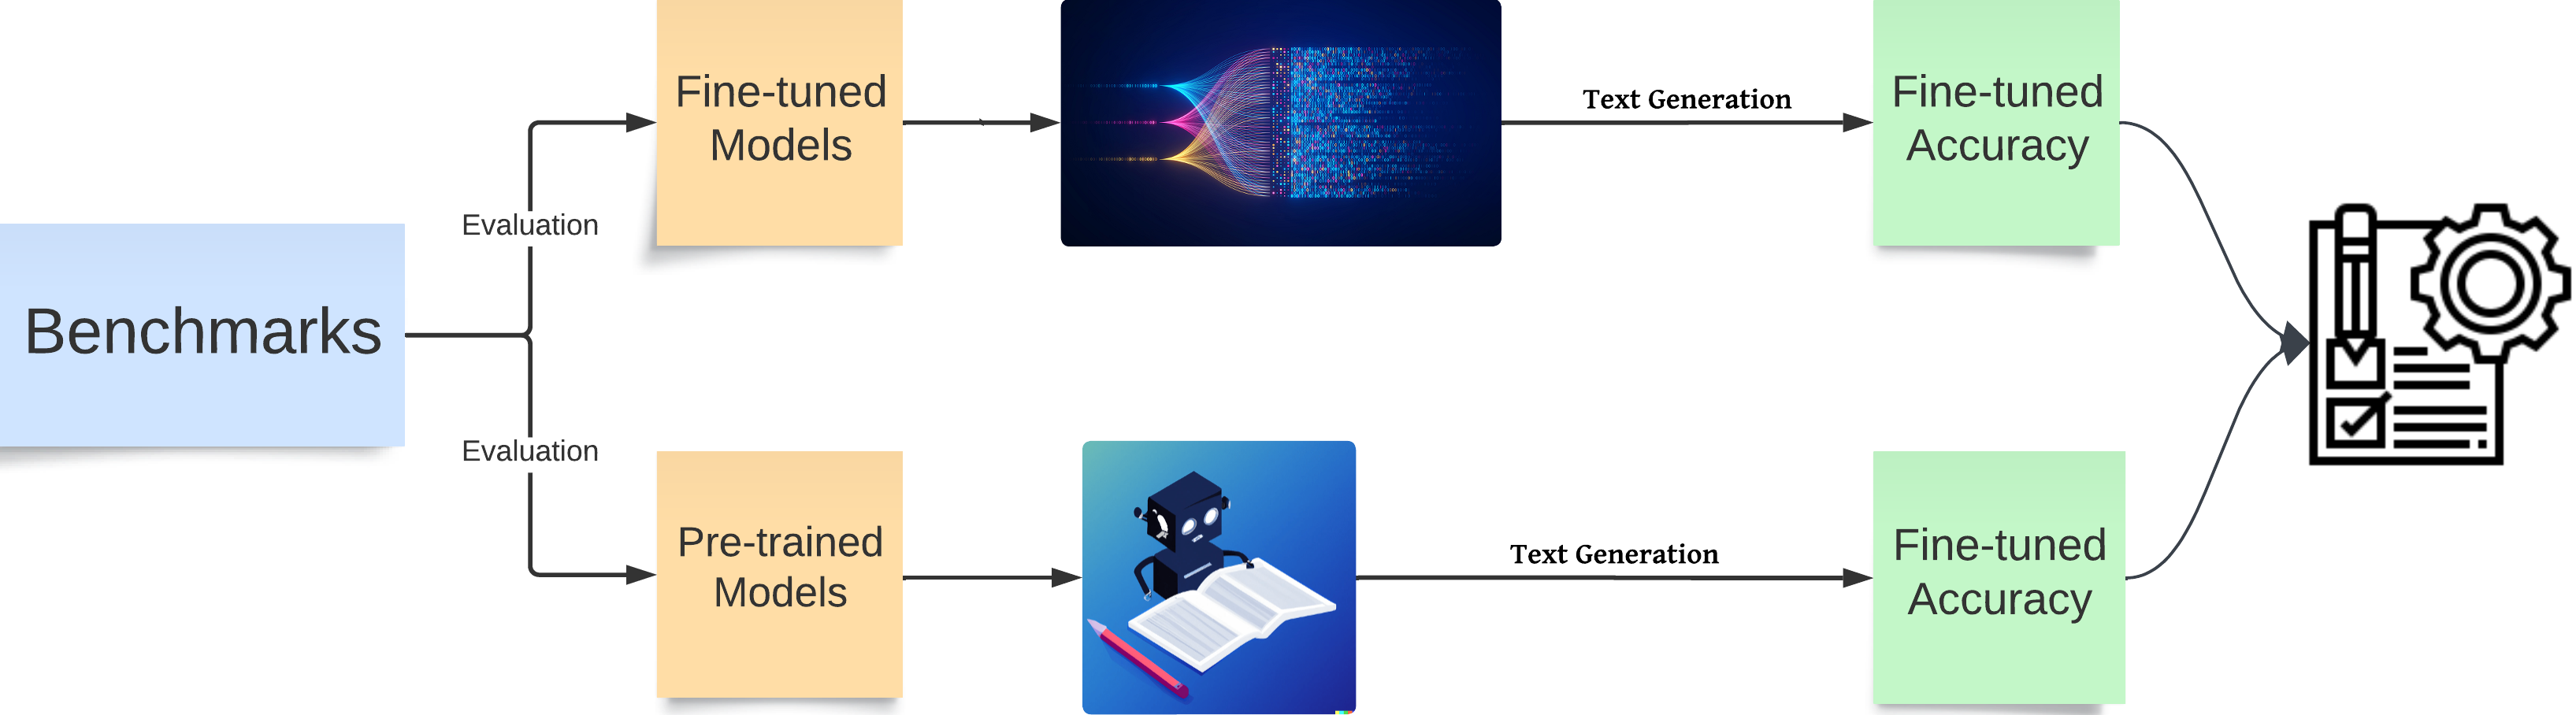
\includegraphics[width=\linewidth]{Figures/Workflow.png}
    \caption{Workflows of our experiment}
    \label{fig:Workflow}
\end{figure}
 
Initially, we deployed the pre-trained models on Google Colab utilizing an A100 GPU with 40GB of RAM and evaluated their performance on our predefined benchmarks in Table \ref{tab:benchmark}. Subsequently, we fine-tuned these models using AI-generated mathematical datasets and evaluated their performance on benchmarks to observe improvements as Figure \ref{fig:Workflow}. We focused on two key metrics to assess the performance of the fine-tuned models:
\begin{itemize}
    \item Accuracy: The primary metric in mathematical QA tasks about calculations and proofs. While some linear algebra and abstract algebra problems necessitate theoretical proofs, evaluating the reasonability of these answers often involves assessing the accuracy of generated answers and logical steps of the proof. 
    \item Cost-Effectiveness: To enable individuals to train personalized mathematical SLMs tailored to spcific requirements as discussed in  section \ref{sec:1}, the cost of computational resources of fine-tuning models and accessing synthesized high quality data would be a crucial metric to justify the feasibility. 
    
\end{itemize}

\subsection{Base Models}\label{sec: model}
We fine-tuned a diverse set of base language models: open-sourced small language models like \textsc{LLama-2-7B/13B} and \textsc{Mistral} due to efficiency of deployment and free of charge; and close-sourced models such as \textsc{GPT-3.5-Turbo} since OpenAI has provided available fine-tuning pipelines and affordable pricing. \\
\\
\textbf{\textsc{LLAMA-2-7B/13B}} \cite{Touvron2023Llama2O} are open-sourced auto-regressive models developed by Meta with 2 trillion pretraining tokens, 4092 context lengths, and over 100K fine-tuning data.\\
\\
\textbf{\textsc{Mistral-7B-v0.1}} \cite{jiang2023mistral7b} is an open-sourced model developed by Mistral AI with the usage of Grouped-Query Attention \cite{ainslie2023gqatraininggeneralizedmultiquery}, Sliding-Window Attention \cite{hassani2023neighborhoodattentiontransformer}, and Byte-fallback BPE tokenizer \cite{Berglund_2023} techniques to enhance the efficiency and performance of the model on many NLP tasks.\\
\\
\textbf{\textsc{Bloom-7B1}} \cite{bigscience2023bloom7b1} is a multilingual SLM developed by BigScience which is a decoder-only model modified from \textsc{Megatron-LM GPT2} \cite{shoeybi2020megatronlmtrainingmultibillionparameter} and was trained using 8-bit optimizers \cite{dettmers20228bitoptimizersblockwisequantization} and ALiBI positional encodings \cite{press2022trainshorttestlong}. \\
\\
\textbf{\textsc{GPT-3.5-Turbo}} \cite{OpenAIGPT35TurboFineTuning} is a LLM developed by OpenAI, representing an evolution of the GPT-3 series, in other words, an enhancement of GPT-3 with advanced performance. It covers many NLP tasks including mathematical reasoning and question-answering. 

\subsection{Baseline Evaluation}
Initially, we evaluated the base models' performance on four benchmark datasets using accuracy as the primary metric. Furthermore, we employed the \textsc{GPT-4} model as a classifier to assess the alignment between the benchmark answers and the answers generated by models to quantify the accuracy. Given our focus on the linear algebra capabilities of SLMs, we selected two  benchmark datasets for our baseline assessment: Linear Algebra QA and MATH Linear Algebra.
\begin{table}[ht]
\centering
\renewcommand{\arraystretch}{0.8} % Adjust vertical spacing
\setlength{\tabcolsep}{10pt} % Adjust horizontal spacing
\begin{tabular}{p{6cm} p{6cm} p{2cm}}
\toprule
\textbf{Benchmark} & \textbf{Model} & \textbf{Accuracy} \\
\midrule
MMLU Abstract Algebra 
    & \textsc{GPT-3.5-Turbo} (LLM) & 22.00\% \\
\midrule
Linear Algebra Theorem QA 
    & \textsc{GPT-3.5-Turbo} (LLM) & 9.62\% \\
\midrule
Linear Algebra QA 
    & \textsc{GPT-3.5-Turbo} (LLM) & 31.84\% \\
    & \textsc{LLama-2-7B} (SLM) & 5.83\% \\
    & \textsc{LLama-2-13B} (SLM) & 8.07\% \\
    & \textsc{Mistral-7B-v0.1} (SLM) & 14.80\% \\
    & \textsc{Bloom 7B1} (SLM) & 0.90\% \\
\midrule
MATH Linear Algebra 
    & \textsc{GPT-3.5-Turbo} (LLM) & 8.60\% \\
    & \textsc{LLama-2-7B} (SLM) & 0.30\% \\
    & \textsc{LLama-2-13B} (SLM) & 1.05\% \\
    & \textsc{Mistral-7B-v0.1} (SLM) & 1.95\% \\
    & \textsc{Bloom 7B1} (SLM) & 0.00\% \\
\bottomrule
\end{tabular}
\caption{Accuracy of Language Models on Algebra Benchmarks.}
\label{tab:model-performance}
\end{table}
\\
According to Table \ref{tab:model-performance}, we observed that the SLMs exhibited limitations in linear algebra calculations compared to \textsc{GPT-3.5-Turbo}. This performance disparity might be attributed to the inherent constraints of SLMs in handling complex mathematical reasoning tasks. Furthermore, while model performance generally improves with increasing parameter size \cite{kaplan2020scalinglawsneurallanguage}, our observations suggest that it is not the sole determining factor since the performance of \textsc{Mistral-7B-v0.1} on both benchmarks exceeded \textsc{LLaMa-2-13B}.

\subsection{Finetuning Settings}
  Followed by instruction of Figure~\ref{fig:Finetuning} , we employed \textsc{Huggingface AutoTrain} tool to fine-tune SLMs on NVidia 1xL40S 8 vCPUs and 62GB of memory. By the way, \textsc{AutoTrain} has user-friendly interface and cost-effectiveness which makes it accessible for people without coding experience. \\
\begin{figure}[h]
    \centering
    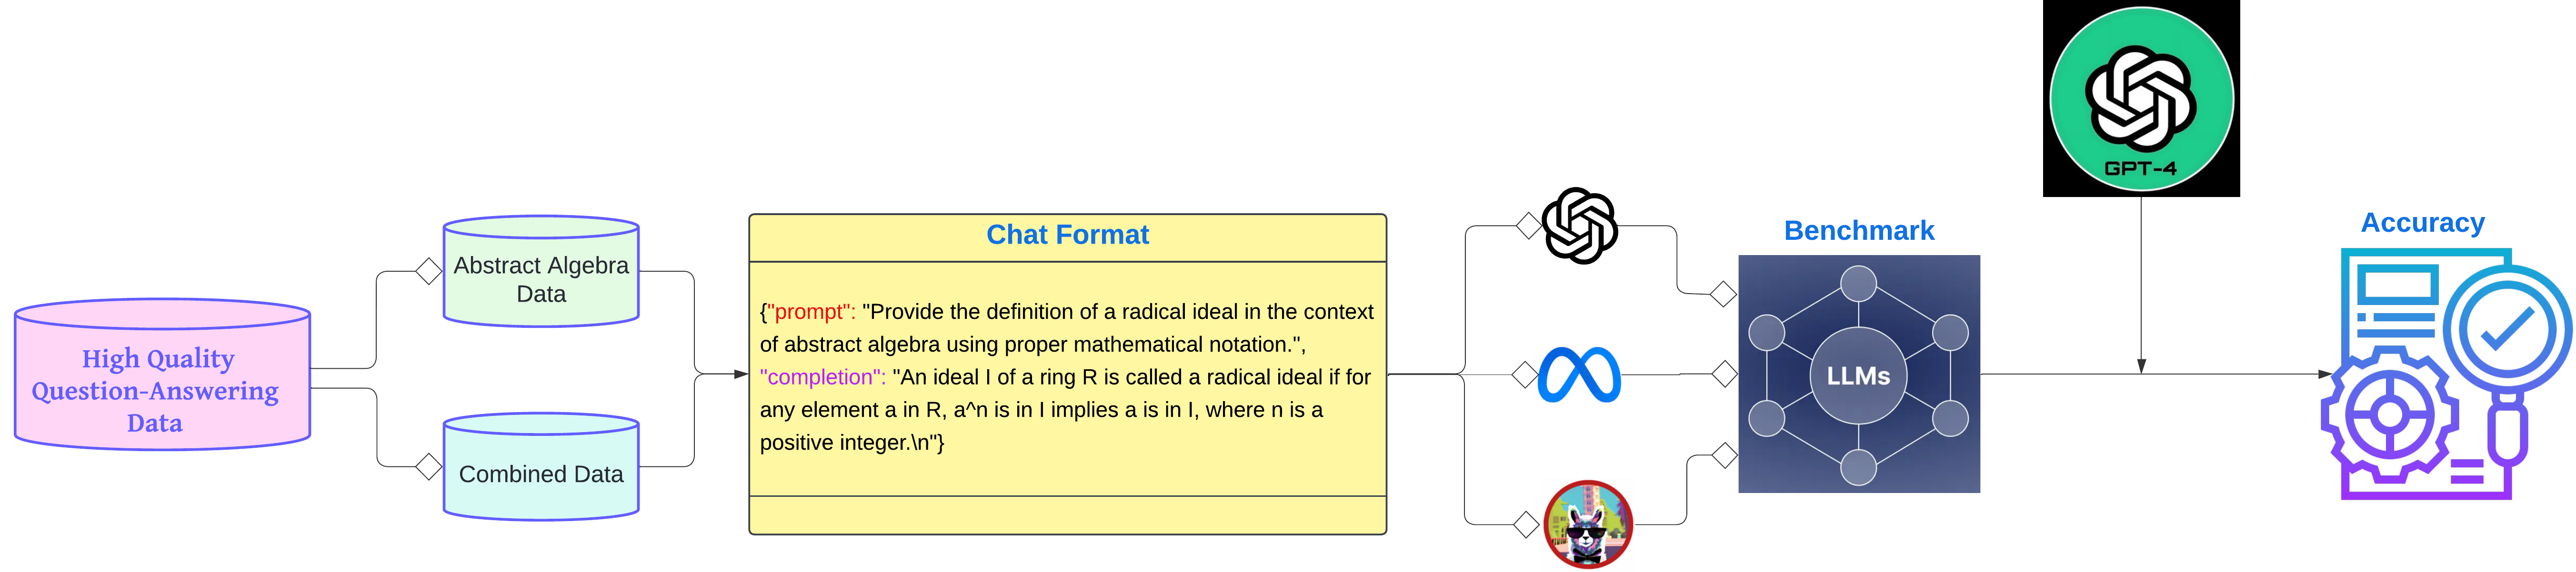
\includegraphics[width=\linewidth]{Figures/Finetuning Process.png}
    \caption{After obtaining the fine-tuning data, we separated them into two subsets: Abstract Algebra and Combined Dataset. Then we used different datasets to fine-tune models and took accuracy as our metric for evaluation according to \textsc{GPT-4} model.}
    \label{fig:Finetuning}
\end{figure}
\\
 
According to \textsc{GPT-3.5-Turbo} requirements of training data format, we converted our CSV data into JSONL format to accommodate GPT chat-model fine-tuning requirements. Subsequently, we utilized OpenAI's API to access its infrastructure to fine-tune models with our synthetic datasets according to instructions of OpenAI Docs. And a well-structured CSV file with a single text column containing questions and corresponding answers would be sufficient for optimal fine-tuning in Autotrain.\\
\\
 
The following hyperparameters used for fine-tuning were employed: 
\begin{itemize}
    \item  \textsc{GPT-3.5-Turbo:} Epochs = 3, Batch size = 6, and Learning rate multiplier = 2. 
    \item \textsc{LLama-2-7b/13b, Bloom 7B1}: Default settings of Autotrain. Chat template = none, Mixed precision = fp16, Optimizer = adamw\_torch, LORA = True, Scheduler = Linear, Batch size = 2, Block size = 1024, Epoches = 3, Gradient accumulation = 4, Learning rate = 0.00003, Model max length = 2048. 
    \item  \textsc{Mistral-7B-v0.1}: We adjusted the hyperparameters from the previous configuration, increasing the batch size to 3 and the number of epochs to 4 for better accommodation of model.
\end{itemize}

  Both the Autotrain and OpenAI's API platforms provided us convenient and efficient fine-tuning approaches for users to train language models.
\subsection{Results}
\begin{figure}[h]
    \centering
    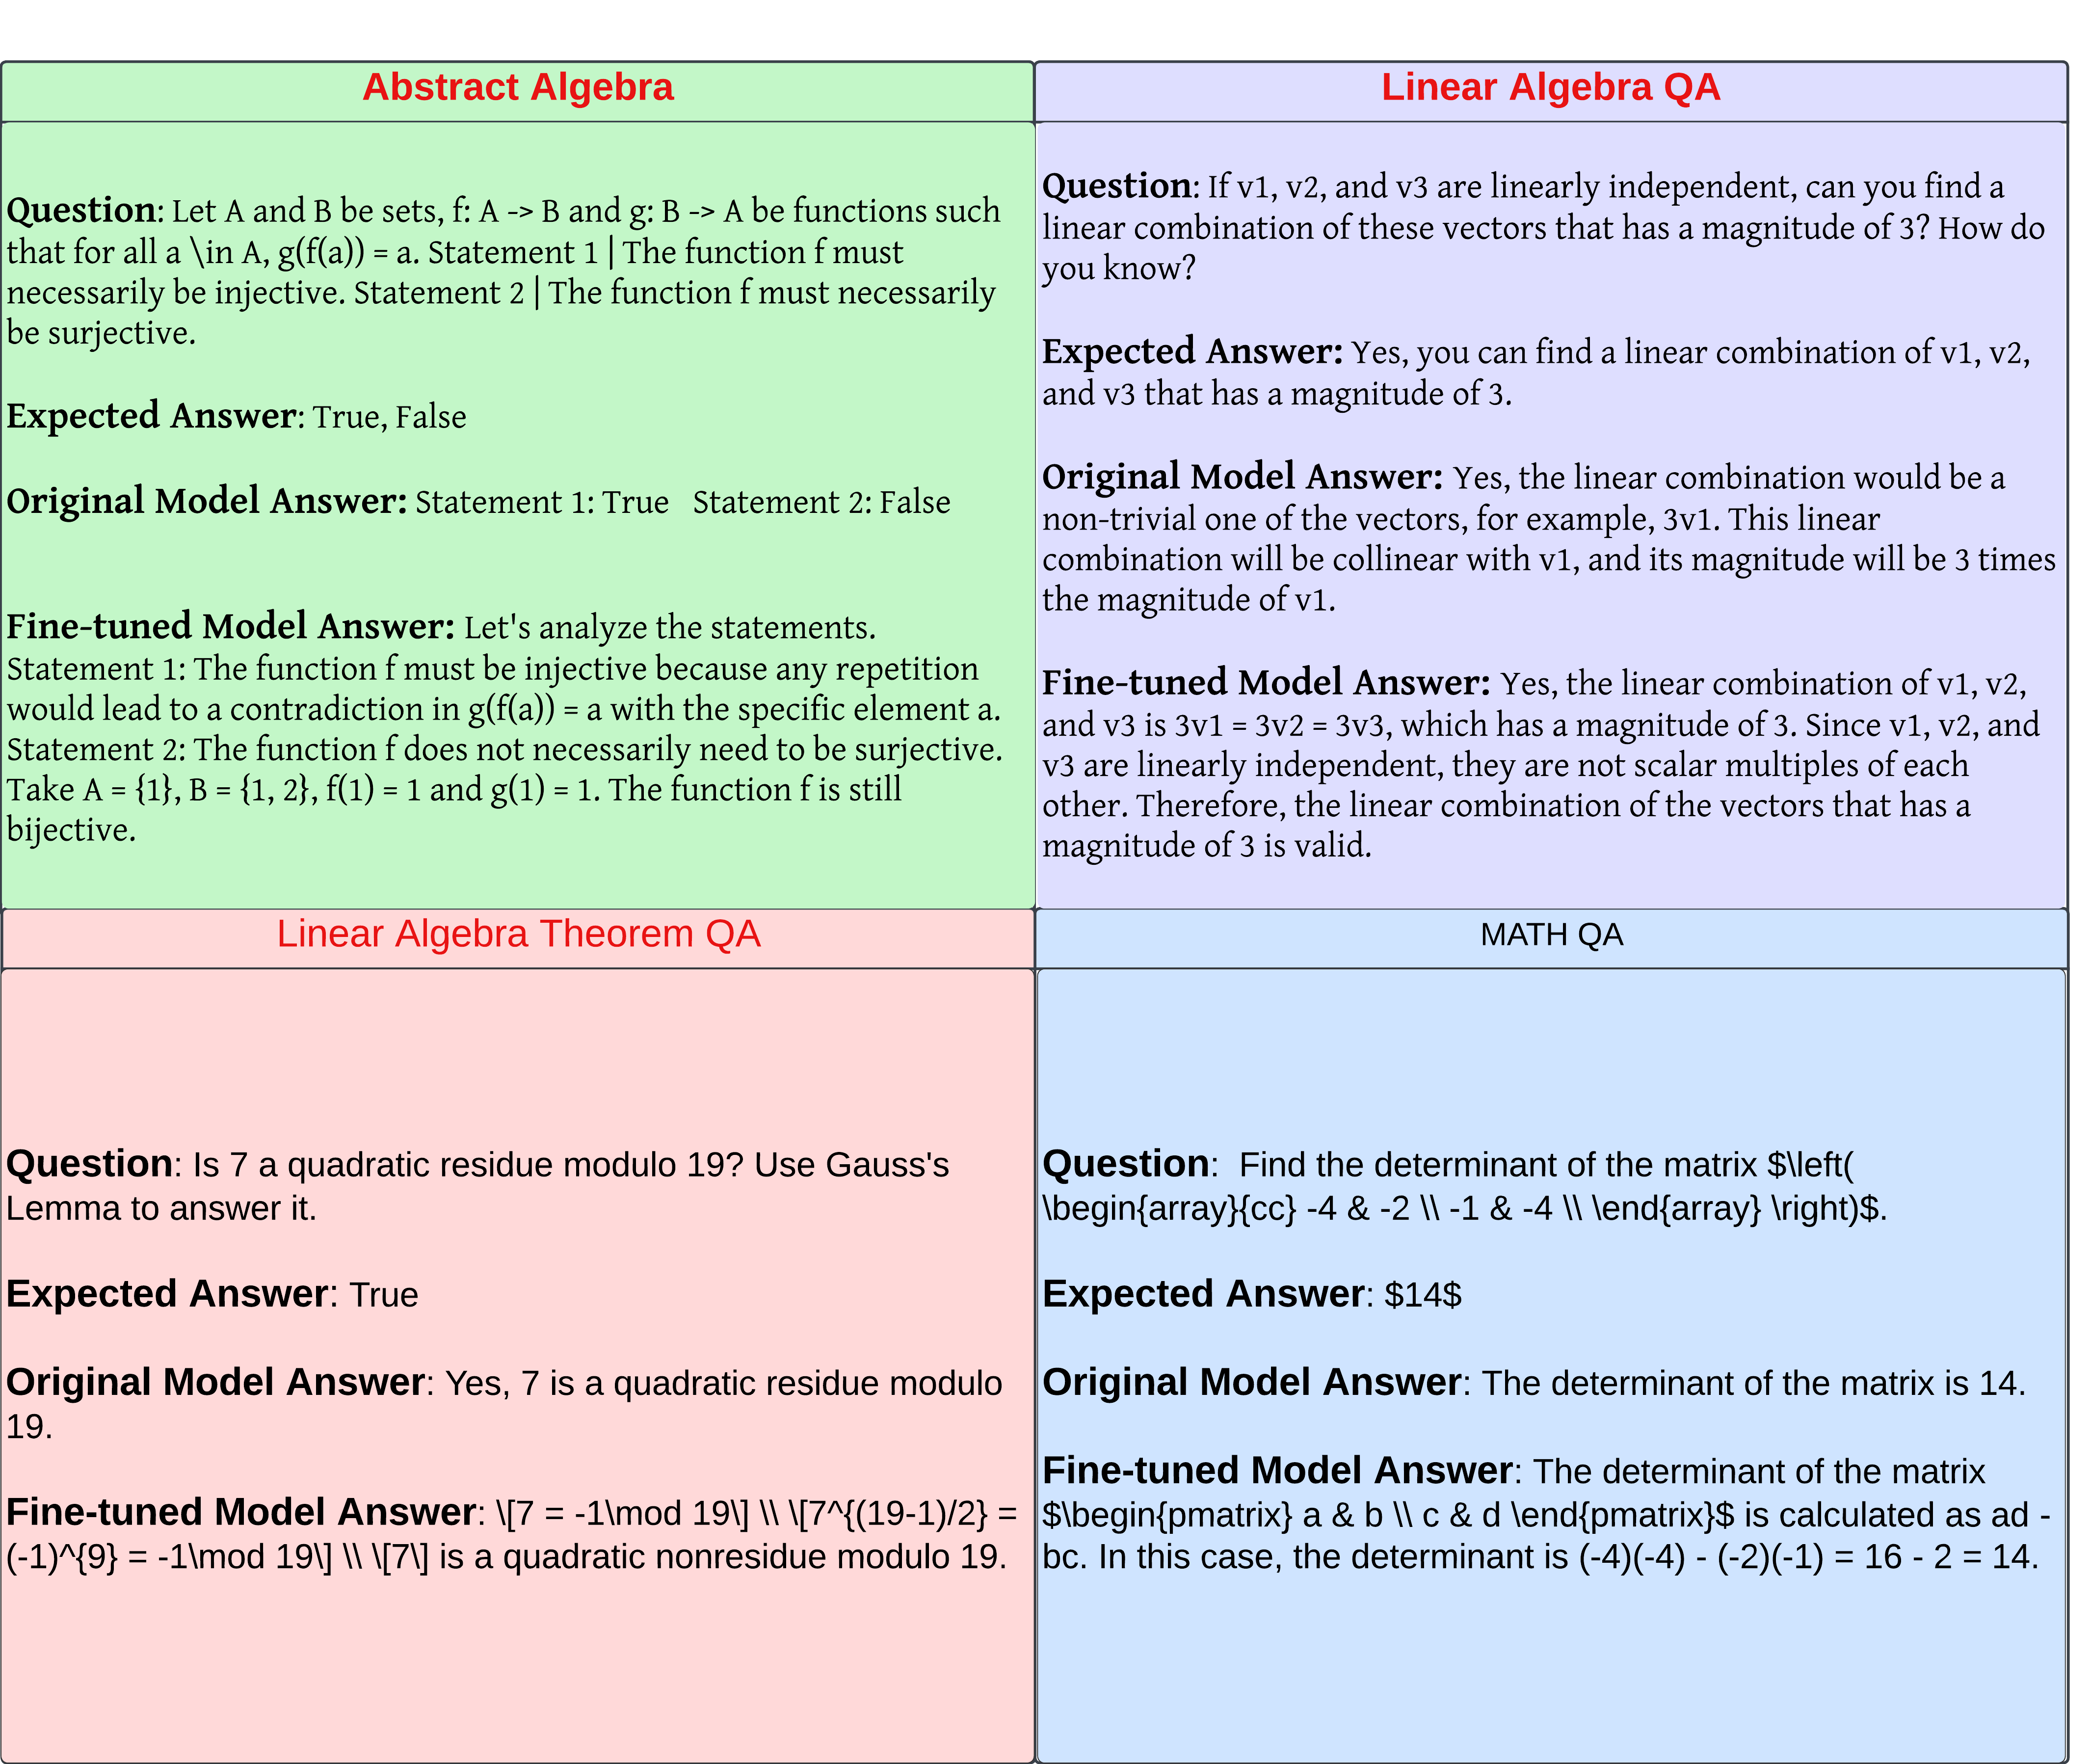
\includegraphics[width=0.6\linewidth]{Figures/Model Outputs.png}
    \caption{The outputs from original and fine-tuned \textsc{GPT-3.5-Turbo} models on benchmarks. Although original model could generate correct answers sometimes, fine-tuned model could provide specific reasoning process and better explanations as our fine-tuned data describes.}
    \label{fig:Outputs}
\end{figure}
 
According to Figure~\ref{fig:Outputs}, we observed that the fine-tuned model not only provided correct answers but also offered explanations, aligning with the Chain-of-Thought reasoning approach \cite{wei2023chainofthoughtpromptingelicitsreasoning}. We fine-tuned the \textsc{GPT-3.5-Turbo} model on two distinct datasets: one consisting exclusively of abstract algebra data, and the other comprising a combination of abstract algebra, linear algebra, and linear algebra calculation data. Both fine-tuned models have performed remarkable progresses on benchmarks. However, as shown in Figure~\ref{fig:Observation}, we unexpectedly observed that the model exclusively fine-tuned on abstract algebra data had an astonishing advancement in \textsc{Linear Algebra QA} benchmark, which surpassed the performance of fine-tuned model on the combined dataset. 

\begin{figure}[h]
    \centering
    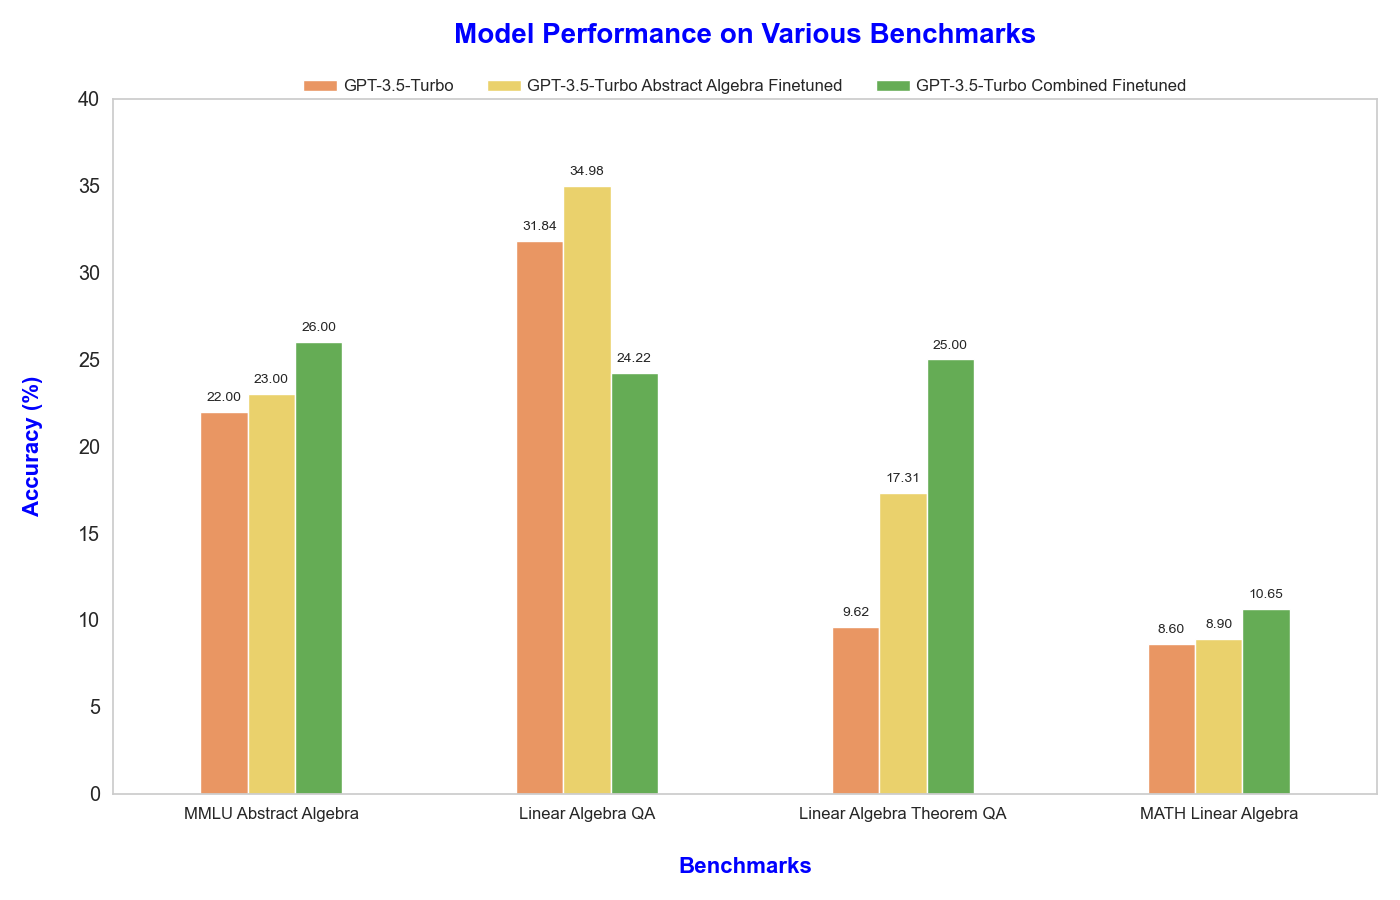
\includegraphics[width=0.8\linewidth]{Figures/GPT-3.5-Turbo_Performance_on_Various_Benchmarks.png}
    \caption{Performance of \textsc{GPT-3.5-Turbo} and its fine-tuned models across various datasets and benchmarks.}
    \label{fig:Observation}
\end{figure}
 
Interestingly, we also observed that fine-tuning \textsc{GPT-3.5 Turbo} model on abstract algebra datasets yielded a notable improvement in accuracy on linear algebra benchmarks, particularly in linear algebra theorem QA as  Figure~\ref{fig:Observation} showed. One of the possible reasons is that the abstract algebra dataset provides the model with a foundational understanding of mathematical structures and concepts that correspond to linear algebra, specifically, vector spaces could be regarded as a group. These two areas exhibit significant overlap in foundational knowledge which enhanced the mathematical inference ability of model in linear algebra tasks.\\ 

\begin{figure}[h]
    \centering
    \begin{subfigure}[b]{0.45\linewidth}
        \centering
        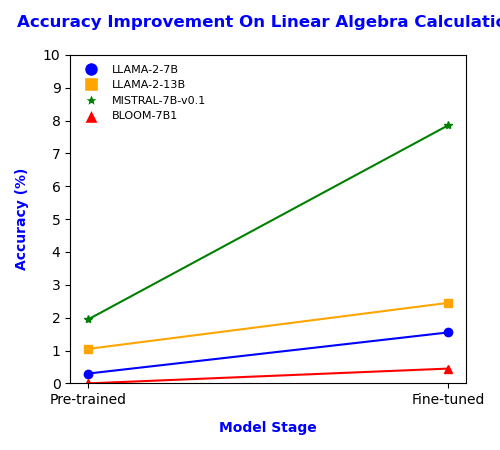
\includegraphics[width=\linewidth]{Figures/Accuracy_Improvement_Calculation.png}
        \caption{Linear Algebra Calculation}
        \label{fig:Accuracy_Calculation}
    \end{subfigure}
    \hfill
    \begin{subfigure}[b]{0.45\linewidth}
        \centering
        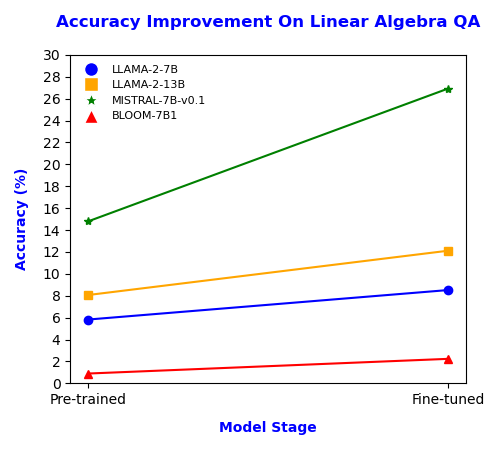
\includegraphics[width=\linewidth]{Figures/Accuracy_Improvement_of_QA.png}
        \caption{Linear Algebra QA}
        \label{fig:Accuracy_QA}
    \end{subfigure}
    \caption{The alternation of accuracy of SLMs on Linear Algebra Calculation and Linear Algebra QA benchmark after fine-tuning on our datasets in section \ref{sec:data}.}
    \label{fig:Accuracy_Improvements}
\end{figure}

Subsequently, we fine-tuned the SLMs and evaluate their performance on Linear Algebra Calculation and Linear Algebra QA benchmarks which demonstrated reasonable improvements in mathematical reasoning ability as Figure~\ref{fig:Accuracy_Improvements} showed. As shown in Figure~\ref{fig:Accuracy_Calculation} and Figure~\ref{fig:Accuracy_QA}, we observed that the \textsc{Mistral-7B-v0.1} \cite{jiang2023mistral7b} model exhibited best improvements of accuracy on both benchmarks after fine-tuning. Its superior performance might be attributed to its advanced architectures of transformers and attention mechanisms as we mentioned in Section~\ref{sec: model}, and its modification of FlashAttention \cite{Dao2022FlashAttentionFA} and xFormers \cite{xformers} makes training procedures faster. 

\section{Cost}
In our experiments, fine-tuning \textsc{GPT-3.5-Turbo} through OpenAI's API infrastructure had a cost of \$5.53 based to its token-based pricing. In contrast, fine-tuning Llama-2 SLMs through Hugging Face's Autotrain platform required only \$0.96 and 32 minutes for the 7B model, and \$3.15 and 105 minutes for the 13B model, which is more cost-effective than \textsc{AlpaGasus} \cite{Chen2023AlpaGasusTA}. Similarly, fine-tuning \textsc{Mistral-7B-v0.1} cost \$1.05 and took 31 minutes, while fine-tuning \textsc{Bloom 7B1} cost \$1.05 and took 35 minutes. Notably, according to Figure~\ref{fig:performance},  \textsc{Mistral-7B-v0.1} is the most fine-tuning effective model due to its remarkable performance on benchmarks with similar costs and fine-tuning time of \textsc{LLama-2-7B} and \textsc{Bloom 7B1} models. 
\begin{figure}[h]
    \centering
    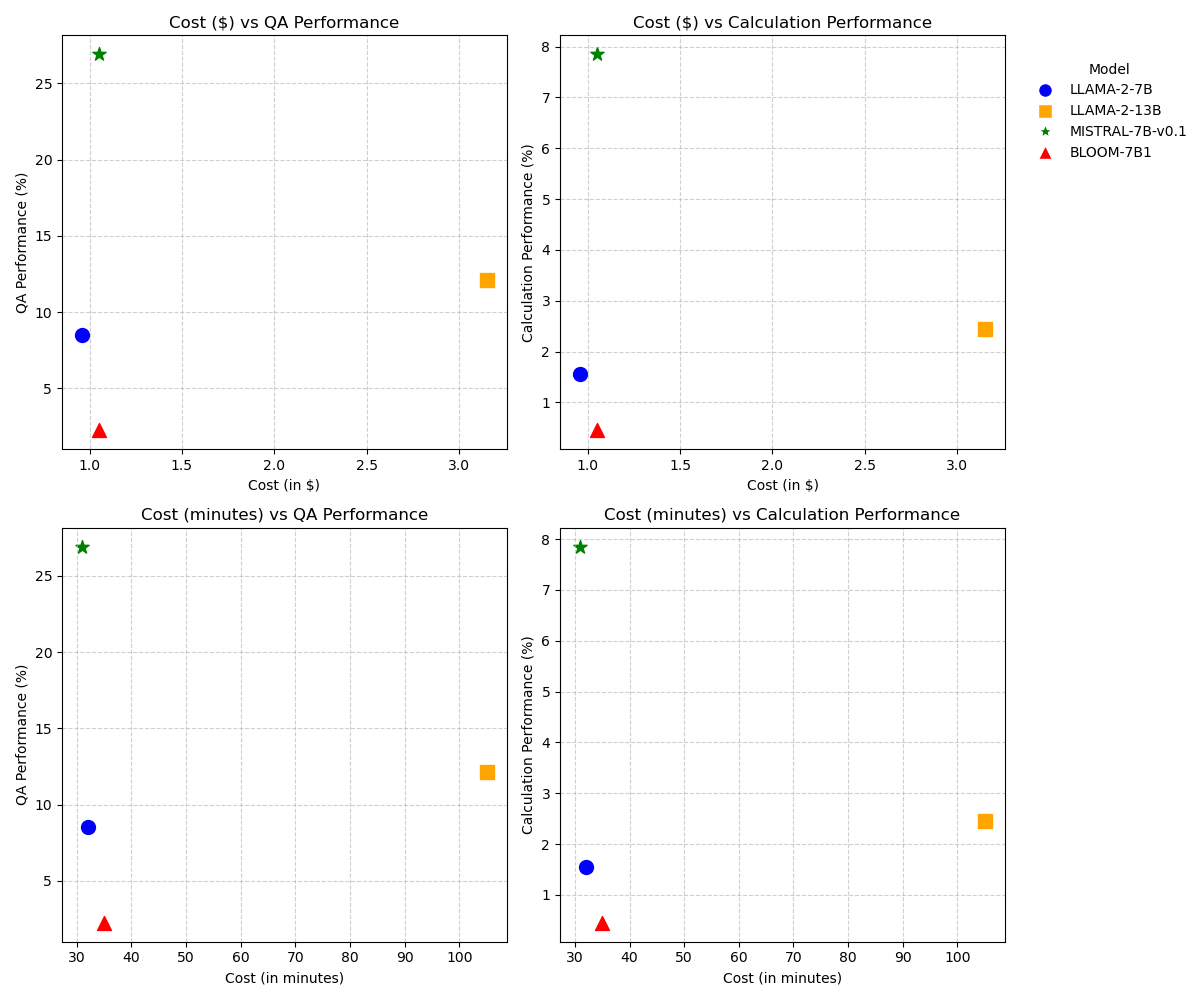
\includegraphics[width=0.8\linewidth]{Figures/Cost_vs_Performance.png}
    \caption{Performance of SLMs and their performance on different benchmarks.}
    \label{fig:performance}
\end{figure}

The low costs of our fine-tuning procedures for SLMs is mainly attributed to efficient application of LoRA \cite{Hu2021LoRALA} which significantly reduced the computational burden of fine-tuning. This highlights how individuals could leverage our method through Autotrain to affordably design and customize language models for their own purposes.

\section{Conclusion}
In conclusion, our method provides a feasible approach to fine-tune mathematical QA language models using synthetic data. Our cost-effective fine-tuning method yielded notable improvements in linear algebra calculations and formulas across various models, including LLMs (e.g., \textsc{GPT-3}) and SLMs (e.g., \textsc{LLama-2-7B} and \textsc{Mistral-7B-v0.1}). Considering the trade-off between cost and performance in fine-tuning, selecting an appropriate pretrained model is crucial to achieve practical usability. Advanced pre-trained SLM tend to have superior performance after fine-tuning, while requiring less costs and time. Our study indicates that synthetic data could be an effective and efficient approach for enhancing the mathematical reasoning capabilities of language models, and our method offers individuals a potentially optimal choice to deploy their own fine-tuning tasks.  

\section{Limitations}
Our study represents a basic exploration into fine-tuning language models with synthetic mathematical data, demonstrating the potential of this approach for enhancing mathematical reasoning and developing personalized models. However, several avenues warrant future investigation to improve the generalization and performance of models. On the one hand, future work should explore incorporating a broader range of mathematical data types, including topology, calculus, and geometry, to enhance the generalization capabilities of the fine-tuned models. On the other hand, exploring more advanced base language models, such as \textsc{Falcon-7B}, could provide greater capacity for solving complex mathematical questions.

\newpage
\printbibliography


\end{document}
